\exam{2023}
\begin{problem}{Poisson Process}
Consider a Poisson process with rate $\lambda$. Let $T_n$ be the time of the $n$-th arrival. Consider a second arrival process and denote $Z_n$ as the time of the $n$-th arrival of this second arrival process. Assume $Z_n$ = c$T_n$ for some constant c $>$ 0. What can you say about this second arrival process? Prove your answer. What do we know about the superposition of these two arrival processes?
\end{problem}

\begin{solution} 
The inter-arrival time of the first process ($T_n - T_{n-1})$ with mean $\frac{1}{\lambda}$ is independent of the second process $ c.(T_n - T_{n-1})$ , with mean $\frac{c}{\lambda}$. We can deduce that the second process is a Poisson process with a scaled rate of $\frac{\lambda}{c}$. 

Furthermore, looking at the superposition of the two arrival processes, we know that the combination of two Poisson processes is just another Poisson process. In this case a Poisson process with arrival rate:
\begin{align*}
    \lambda +\frac{\lambda}{c}= \lambda\left (1+\frac{1}{c}  \right )
\end{align*}
\end{solution}

\begin{problem}{Discrete-Time Markov Chains}
Given a DTMC with state space S such that state i = 1 has period $d_1$ = 3, state i = 2 has period $d_2$ = 5 and there are at least 3 open communicating classes. What is the smallest possible value for $| S |$  ? Explain your answer. Give an example (by defining P) of a DTMC such that $| S |$ is minimized
\end{problem}

\begin{problem}{Discrete-Time Markov Chains}
Assume we flip a coin infinitely often. How many coin flips do we need on average until we flipped the sequence HTH (heads-tails-heads)? Explain your answer.
\end{problem}

\begin{solution}
  We can model this problem as a DTMC where each transition has a probability of $\frac{1}{2}$. Each state represents a step in the sequence. We now calculate the mean hitting time for $A = \{3\}$, where state 3 represents the successful observation of "HTH."

  \begin{figure}[h!]
    \begin{center}
      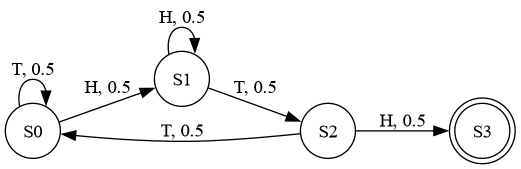
\includegraphics[width=0.5\textwidth]{img/23.2.png}
    \end{center}
    \caption{DTMC modelling coin flips to reach an HTH sequence}
  \end{figure}

  \textbf{Remember:} Let $\{X_n, n \geq 0\}$ be a Markov chain characterized by transition matrix $P$, and let $A \subseteq S$ be a subset of states. Then, the mean hitting times $k^A_i$ of $A$ are the smallest non-negative solution to:
  \[
    x_i =
    \begin{cases}
      0, & i \in A, \\
      1 + \sum_{j \notin A} p_{i,j} x_j, & i \notin A.
    \end{cases}
  \]

  Define \( x_i \) as the mean hitting time (expected number of flips) to reach state 3 from state \( i \).

  \begin{itemize}
    \item $x_3 = 0$ since $3 \in A$, which is our target state.
    \item For $x_0$ (starting from the initial state):
      \[
        x_0 = 1 + \frac{1}{2}x_1 + \frac{1}{2}x_0
      \]
      Rearranging, we get:
      \[
        \frac{1}{2}x_0 = 1 + \frac{1}{2}x_1
      \]
      \[
        x_0 = 2 + x_1
      \]

    \item For $x_1$ (starting from the state where "H" is observed):
      \[
        x_1 = 1 + \frac{1}{2}x_2 + \frac{1}{2}x_1
      \]
      Rearranging, we get:
      \[
        \frac{1}{2}x_1 = 1 + \frac{1}{2}x_2
      \]
      \[
        x_1 = 2 + x_2
      \]

    \item For $x_2$ (starting from the state where "HT" is observed):
      \[
        x_2 = 1 + \frac{1}{2}x_3 + \frac{1}{2}x_0
      \]
      Simplifying, since \( x_3 = 0 \):
      \[
        x_2 = 1 + \frac{1}{2}x_0
      \]
  \end{itemize}

  We now solve this system of equations step-by-step:

  \begin{enumerate}
    \item Substitute \( x_1 = 2 + x_2 \) into \( x_0 = 2 + x_1 \):
      \[
        x_0 = 4 + x_2
      \]
    \item Substitute \( x_0 = 4 + x_2 \) into \( x_2 = 1 + \frac{1}{2}x_0 \)
      \[
        x_2 = 1 + \frac{1}{2}\left( 4 + x_2 \right)
      \]
      \[
        \frac{1}{2}x_2 = 3
      \]
      \[
        x_2 = 6
      \]
    \item Substitute \( x_2 = 6 \) into \( x_0 = 4 + x_2 \):
      \[
        x_0 = 4 + 6 = 10
      \]
  \end{enumerate}

  Thus, the mean hitting time to reach the sequence "HTH" (state 3) from the starting state (state 0) is:
  \[
  \boxed{x_0 = 10}
  \]
  Therefore, on average, it takes 10 coin flips to observe the sequence "HTH" for the first time.
\end{solution}

\begin{problem}{Continuous-Time Markov Chains}
Consider an infinite state continuous-time Markov chain (CTMC) with state space $\{0, 1, 2, \ldots\}$ and rate matrix $Q$, such that for $i \neq j$ we have:

\[
q_{i,j} =
\begin{cases}
    q_{i,i+1} & \text{if } i \text{ is odd, } j = i + 1, \\
    q_{i,i+3} & \text{if } i \text{ is odd, } j = i + 3, \\
    q_{i,i-1} & \text{if } i > 0 \text{ is even, } j = i - 1, \\
    q_{i,i-3} & \text{if } i > 0 \text{ is even, } j = i - 3, \\
    q_{0,2} & \text{if } i = 0, j = 2, \\
    q_{2,0} & \text{if } i = 2, j = 0, \\
    0 & \text{otherwise.}
\end{cases}
\]

Let $(\pi_0, \pi_1, \ldots)$ be its invariant distribution. Give an explicit expression for $\frac{\pi_{13}}{\pi_0}$. 

Explain your answer.
\end{problem}

\begin{problem}{Applications}
    Consider an M/M/1 queue with arrival rate $\lambda$ and service rate $\mu > \lambda$. Assume a job is labelled type-1 upon arrival with probability $p$ and type-2 otherwise. Jobs are labelled independent of each other. Instead of serving the jobs in FCFS order, type-1 jobs get priority over type-2 jobs. A type-2 job can only be in service if no type-1 jobs are present and is interrupted (and resumed later) if a type-1 job arrives. What is the mean response time of a type-1 job in such a system? Explain. Derive an expression for the mean response time of a type-2 job.
\end{problem}

\begin{problem}{Applications}
   Consider a Jackson network with $M = 4$ queues and $\mu_1 = \mu_2 = \mu_3 = \mu_4 = 1$. All new arrivals either join queue 1 or 2 (with equal probability). The routing probabilities are as follows: $ p_{1,3} = p_{1,4} = \frac{1}{2}$, $p_{2,3} = \frac{1}{8}$, $p_{2,4} = \frac{7}{8}$, $p_{4,0} = 1$, $p_{3,3} = p_{3,0} = \frac{1}{2}$. State a necessary and sufficient condition such that the Markov chain of the joint queue lengths is positive recurrent. For which of these 4 queues is the input process Poisson? Derive an expression for the probability that both queue 3 and 4 are empty at the same time.
\end{problem}

\begin{problem}{Applications}
   In which of the following two systems is the blocking probability the largest: (1) an Erlang-B system with arrival rate $\lambda$, mean call duration $\frac{1}{\mu}$ and $C$ lines or (2) an Engset system with $\lambda' = \frac{\lambda}{N}$, mean call duration $\frac{1}{\mu}$ and $C$ lines? Explain.
\end{problem}
